% ==============================================================================
% COLOR DEFINITIONS FOR 7 ABLATION VARIANTS (Place in Preamble or before figure)
% ==============================================================================
\definecolor{colorhybrid}{RGB}{31, 119, 180}    % Trinity (Full): Strong Blue
\definecolor{coloradam}{RGB}{127, 127, 127}     % Adam (Baseline): Muted Gray
\definecolor{colororange}{RGB}{255, 127, 14}    % w/o K-FAC (SO off): Orange
\definecolor{colorpurple}{RGB}{148, 103, 189}   % Always-On K-FAC: Purple
\definecolor{colorred}{RGB}{214, 39, 40}        % w/o Magnitude Grafting: Red
\definecolor{colorbrown}{RGB}{140, 86, 75}      % w/o Grad. Centralization: Brown
\definecolor{colorteal}{RGB}{23, 190, 207}      % w/o Saddle Escape: Teal

% ==============================================================================
% FIGURE: 3 ABLATION LOSS PLOTS (7 LINES EACH) CALLING CSVs
% ==============================================================================
\begin{figure*}[!t]
  \centering
  % --- SUBFIGURE (a): Wide-ResNet-101-2 ---
  \begin{subfigure}[b]{0.32\textwidth}
    \centering
    \begin{tikzpicture}
      \begin{axis}[
        width=\textwidth,
        height=4.8cm,
        ymode=log,
        title={\textbf{Wide-ResNet-101-2 (Exp.\,1)}},
        title style={font=\small, yshift=-2pt},
        xlabel={Epoch},
        ylabel={Training Loss},
        xlabel style={font=\footnotesize, yshift=2pt},
        ylabel style={font=\footnotesize, xshift=-2pt},
        tick label style={font=\scriptsize},
        xmin=1, xmax=200,
        ymin=0.0001, ymax=4.0,
        xtick={1,50,100,150,200},
        grid=both,
        minor grid style={line width=0.2pt, draw=black!5},
        major grid style={line width=0.4pt, draw=black!12, dashed},
      ]
      \addplot[line width=1.1pt, color=coloradam, dashed, mark=none] table [x=epoch, y=loss, col sep=comma] {CSVs_ablation/exp1_adam.csv};
      \addplot[line width=1.3pt, color=colorhybrid, mark=none] table [x=epoch, y=loss, col sep=comma] {CSVs_ablation/exp1_trinity_full.csv};
      \addplot[line width=1.0pt, color=colororange, dashdotted, mark=none] table [x=epoch, y=loss, col sep=comma] {CSVs_ablation/exp1_without_kfac.csv};
      \addplot[line width=1.1pt, color=colorpurple, mark=none] table [x=epoch, y=loss, col sep=comma] {CSVs_ablation/exp1_kfac_always_on.csv};
      \addplot[line width=1.0pt, color=colorred, densely dotted, mark=none] table [x=epoch, y=loss, col sep=comma] {CSVs_ablation/exp1_no_grafting.csv};
      \addplot[line width=1.0pt, color=colorbrown, densely dashed, mark=none] table [x=epoch, y=loss, col sep=comma] {CSVs_ablation/exp1_no_gc.csv};
      \addplot[line width=1.0pt, color=colorteal, dashdotdotted, mark=none] table [x=epoch, y=loss, col sep=comma] {CSVs_ablation/exp1_no_escape.csv};
      \end{axis}
    \end{tikzpicture}
    \caption{Wide-ResNet-101-2}
    \label{fig:ablation_loss_wrn}
  \end{subfigure}
  \hfill
  % --- SUBFIGURE (b): Vision Transformer ---
  \begin{subfigure}[b]{0.32\textwidth}
    \centering
    \begin{tikzpicture}
      \begin{axis}[
        width=\textwidth,
        height=4.8cm,
        ymode=log,
        title={\textbf{Vision Transformer (Exp.\,2)}},
        title style={font=\small, yshift=-2pt},
        xlabel={Epoch},
        ylabel={Training Loss},
        xlabel style={font=\footnotesize, yshift=2pt},
        ylabel style={font=\footnotesize, xshift=-2pt},
        tick label style={font=\scriptsize},
        xmin=1, xmax=200,
        ymin=0.00005, ymax=4.0,
        xtick={1,50,100,150,200},
        grid=both,
        minor grid style={line width=0.2pt, draw=black!5},
        major grid style={line width=0.4pt, draw=black!12, dashed},
      ]
      \addplot[line width=1.1pt, color=coloradam, dashed, mark=none] table [x=epoch, y=loss, col sep=comma] {CSVs_ablation/exp2_adam.csv};
      \addplot[line width=1.3pt, color=colorhybrid, mark=none] table [x=epoch, y=loss, col sep=comma] {CSVs_ablation/exp2_trinity_full.csv};
      \addplot[line width=1.0pt, color=colororange, dashdotted, mark=none] table [x=epoch, y=loss, col sep=comma] {CSVs_ablation/exp2_without_kfac.csv};
      \addplot[line width=1.1pt, color=colorpurple, mark=none] table [x=epoch, y=loss, col sep=comma] {CSVs_ablation/exp2_kfac_always_on.csv};
      \addplot[line width=1.0pt, color=colorred, densely dotted, mark=none] table [x=epoch, y=loss, col sep=comma] {CSVs_ablation/exp2_no_grafting.csv};
      \addplot[line width=1.0pt, color=colorbrown, densely dashed, mark=none] table [x=epoch, y=loss, col sep=comma] {CSVs_ablation/exp2_no_gc.csv};
      \addplot[line width=1.0pt, color=colorteal, dashdotdotted, mark=none] table [x=epoch, y=loss, col sep=comma] {CSVs_ablation/exp2_no_escape.csv};
      \end{axis}
    \end{tikzpicture}
    \caption{Vision Transformer}
    \label{fig:ablation_loss_vit}
  \end{subfigure}
  \hfill
  % --- SUBFIGURE (c): ResNet-18 ---
  \begin{subfigure}[b]{0.32\textwidth}
    \centering
    \begin{tikzpicture}
      \begin{axis}[
        width=\textwidth,
        height=4.8cm,
        ymode=log,
        title={\textbf{ResNet-18 (Exp.\,3)}},
        title style={font=\small, yshift=-2pt},
        xlabel={Epoch},
        ylabel={Training Loss},
        xlabel style={font=\footnotesize, yshift=2pt},
        ylabel style={font=\footnotesize, xshift=-2pt},
        tick label style={font=\scriptsize},
        xmin=1, xmax=200,
        ymin=0.0005, ymax=4.0,
        xtick={1,50,100,150,200},
        grid=both,
        minor grid style={line width=0.2pt, draw=black!5},
        major grid style={line width=0.4pt, draw=black!12, dashed},
      ]
      \addplot[line width=1.1pt, color=coloradam, dashed, mark=none] table [x=epoch, y=loss, col sep=comma] {CSVs_ablation/exp3_adam.csv};
      \addplot[line width=1.3pt, color=colorhybrid, mark=none] table [x=epoch, y=loss, col sep=comma] {CSVs_ablation/exp3_trinity_full.csv};
      \addplot[line width=1.0pt, color=colororange, dashdotted, mark=none] table [x=epoch, y=loss, col sep=comma] {CSVs_ablation/exp3_without_kfac.csv};
      \addplot[line width=1.1pt, color=colorpurple, mark=none] table [x=epoch, y=loss, col sep=comma] {CSVs_ablation/exp3_kfac_always_on.csv};
      \addplot[line width=1.0pt, color=colorred, densely dotted, mark=none] table [x=epoch, y=loss, col sep=comma] {CSVs_ablation/exp3_no_grafting.csv};
      \addplot[line width=1.0pt, color=colorbrown, densely dashed, mark=none] table [x=epoch, y=loss, col sep=comma] {CSVs_ablation/exp3_no_gc.csv};
      \addplot[line width=1.0pt, color=colorteal, dashdotdotted, mark=none] table [x=epoch, y=loss, col sep=comma] {CSVs_ablation/exp3_no_escape.csv};
      \end{axis}
    \end{tikzpicture}
    \caption{ResNet-18}
    \label{fig:ablation_loss_resnet18}
  \end{subfigure}

  \vspace{4pt}
  % --- SHARED LEGEND ---
  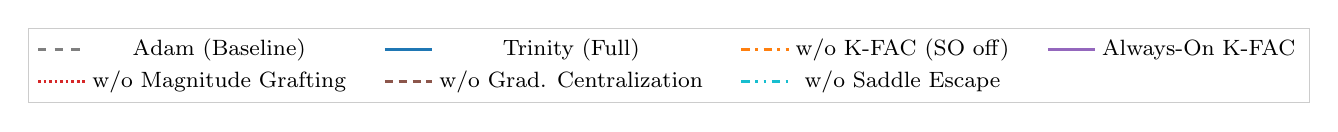
\begin{tikzpicture}
    \begin{axis}[
      hide axis,
      xmin=10, xmax=50, ymin=0, ymax=0.4,
      legend columns=4,
      legend style={
        draw=black!20,
        fill=white,
        font=\footnotesize,
        /tikz/every even column/.append style={column sep=0.4cm}
      }
    ]
    \addlegendimage{line width=1.1pt, color=coloradam, dashed}
    \addlegendentry{Adam (Baseline)}
    \addlegendimage{line width=1.3pt, color=colorhybrid}
    \addlegendentry{Trinity (Full)}
    \addlegendimage{line width=1.0pt, color=colororange, dashdotted}
    \addlegendentry{w/o K-FAC (SO off)}
    \addlegendimage{line width=1.1pt, color=colorpurple}
    \addlegendentry{Always-On K-FAC}
    \addlegendimage{line width=1.0pt, color=colorred, densely dotted}
    \addlegendentry{w/o Magnitude Grafting}
    \addlegendimage{line width=1.0pt, color=colorbrown, densely dashed}
    \addlegendentry{w/o Grad. Centralization}
    \addlegendimage{line width=1.0pt, color=colorteal, dashdotdotted}
    \addlegendentry{w/o Saddle Escape}
    \end{axis}
  \end{tikzpicture}

  \caption{Systematic component ablation study: Training Loss convergence trajectories across 200 epochs on Long-Tailed CIFAR-10 ($\text{IF}=0.01$) for all seven ablation configurations across (a) Wide-ResNet-101-2, (b) Vision Transformer, and (c) ResNet-18.}
  \label{fig:ablation_loss_curves}
\end{figure*}
